\documentclass[11pt]{exam}
\usepackage[utf8]{inputenc}
\usepackage[margin = 1in]{geometry}

% Language packages
\usepackage[spanish]{babel}
\usepackage{csquotes}

% Figure packages
\usepackage{graphicx}

% Math packages
\usepackage{amsmath, amsfonts}

% Reference packages
\usepackage[
    backend = biber,
    style = apa,
]{biblatex}
\addbibresource{main.bib}

\begin{document}
    \begin{titlepage}
        \centering
        {
\includegraphics[width = 4in]{pictures/itesm-logo.png}\par}
        \vspace{0.4in}
        {\bfseries\LARGE Instituto Tecnol\'ogico y de Estudios Superiores de Monterrey \par}
        \vspace{0.4in}
        {\scshape\Large Laboratorio Integral de Control Automático \par}
        {\Large Dra. Debbie Crystal Hernández Zárate \par}
        {\Large Dra. Marybeth Flores Vázquez \par}
        \vspace{1.2in}
        {\Large ``Sistema de Control para la Eliminaci\'on de Pulg\'on Amarillo, \textit{Melanaphis sacchari}, en Cultivos de Maíz por medio de un Dron Parrot Bebop 2'' \par}
        \vspace{1.2in}
        {\itshape\Large Proyecto \par}
        \vfill
        {\Large Autores: \par}
        {\Large Gerardo Dom\'inguez Ram\'irez\par}
        {\Large Claudia Vanessa Dorantes Villegas\par}
        {\Large Uziel Hernández Espejo\par}
        {\Large Carlos Diego Fernández\par}
        {\Large Emmanuel Ramírez Reyes\par}
        \vfill
        {\Large Diciembre 2022 \par}
    \end{titlepage}

    \header{
\includegraphics[width = 1in]{pictures/itesm-logo.png}}{}{Diciembre 2022}
    \footer{}{P\'agina\ \thepage\ de \numpages}{}
    \headrule
    \footrule

    \section*{Resumen}
        [Texto]
    
    \section{Introducci\'on} \label{sec1}
    La tecnolog\'ia est\'a desempeñando su papel en la globalizaci\'on y los drones presentan un uso cada vez mayor en una amplia gama de disciplinas (\cite{nouacer-2020}). La gran demanda de estos dispositivos se debe a su capacidad para responder a las necesidades de las personas. La mayor\'ia de estos brindan a los una amplia visión por medio de c\'amaras que se pueden activar y usar casi en cualquier lugar y en cualquier momento (\cite{yaacoub-2020}). Por ello sus aplicaciones se encuentran en un amplio rango de áreas, siendo las más relevantes la salud, el ej\'ercito y la agricultura (\cite{ayamga-2021}).

    Las tres revoluciones industriales anteriores transformaron profundamente la industria agr\'icola de la agricultura autóctona a la agricultura mecanizada y la agricultura de precisi\'on reciente (\cite{liu-2020}). Los drones están creando una nueva revolución agr\'icola. Se estima que el tamaño de los drones en el mercado agrícola alcanzar\'a los miles de millones de d\'olares en los pr\'oximos años. Como editor del informe de investigaci\'on de la Organizaci\'on de las Naciones Unidas para la Agricultura y la Alimentación y la Uni\'on Internacional de Telecomunicaciones sobre ``UAV y agricultura'', el experto en informaci\'on Gerard Sylvester dijo que mientras los agricultores trabajan para adaptarse al cambio clim\'atico y enfrentar otros desaf\'ios, se espera que los drones ayuden a todo el sector agr\'icola. las empresas mejoran la eficiencia (\cite{ren-2020}).

    Una de las afecciones más comunes en los campos de cultivo son las plagas y enfermedades que conllevan a bajos rendimientos de producción. Los agricultores se han basado tradicionalmente en métodos manuales para identificar plagas y enfermedades, lo que consume mucho tiempo y es costoso (\cite{xing-2022}). El internet y la omnipresencia de los dispositivos móviles con cámara en drones fungen como una oportunidad para adquisición de imágenes conveniente y económica, así como el uso de modelos de aprendizaje profundo para reconocer plagas y enfermedades en el campo.

    En el caso de M\'exico, los métodos agrícolas tradicionales de pequeñas parcelas trabajadas por familias y pequeñas comunidades contin\'uan dominando en muchas regiones, especialmente en aquellas con grandes poblaciones ind\'igenas como la Meseta Sur (\cite{alvarez-2018}). Muchos a\'un subsisten gracias a la agricultura de autoconsumo y ganan dinero vendiendo los excedentes de cosecha en los mercados locales, especialmente en el centro y sur de México (\cite{negrete-2018}). La automatizaci\'on de la agricultura y la detección y control de riesgos a pequeña y gran escala es de colosal importancia, ya que aplicando tecnolog\'ias mecatr\'onicas a la agricultura ayudar\'ia a detonar la productividad en la agricultura mexicana.

    Es por ello que la presente investigaci\'on tiene como objetivo implementar la simulaci\'on de un sistema de control para la eliminaci\'on de pulg\'on amarillo, \textit{Melanaphis sacchari}, en cultivos de ma\'iz en una regi\'on del territorio mexicano. Esto con la finalidad de acelerar el proceso de identificaci\'on y reducir su costo. Se plantea simular el recorrido del dron a trav\'es del campo de cultivo realizando las capturas necesarias sin perder la trayectoria. En la Secci\'on \ref{sec2} se realiza una investigaci\'on exhaustiva de los sistemas existentes que implementan sistemas de control y realizan procesos de identificaci\'on. En la Secci\'on \ref{sec3} se explica la metodología del sistema de control junto con análisis matemático y trayectorias de exploración en el campo de cultivo. En la Secci\'on \ref{sec4} se presentan los resultados de la simulaci\'on. Y finalmente en la Secci\'on \ref{sec5} se presentan las conclusiones.

    \section{Antecedentes}\label{sec2}
        \subsection{Panorama General del Uso de Drones para el Control de Plagas}\label{sec2.1}
        Los drones son muy \'utiles para detectar problemas en el campo y tomar medidas correctivas al instante. \textcite{subramanian-2021} hallaron que la aplicaci\'on de drones en la agricultura se centra en aplicaciones de pesticidas con investigaci\'on centrada en cultivos de arroz \autocite{quin-2016}, trigo \autocite{wang-2019}, ma\'iz \autocite{zheng-2017}, algod\'on \autocite{lou-2018}, pimienta \autocite{xiao-2020} y caña de az\'ucar \autocite{zhang-2019}, ya que se cultivan en \'areas grandes de bloques contiguos donde la aplicaci\'on de drones es factible y legal. Además, para mejorar la eficiencia del uso de insecticidas en los cultivos, se considera que la altura de vuelo de $2$ a $3\;\mathrm{m}$, la velocidad de vuelo de $3$ a $5\;\mathrm{m/s}$, la boquilla de dos ventiladores, el UAV de cuatro rotores y la carga útil de $15\;\mathrm{l}$ son óptimos para realizar fumigaciones de pesticidas con drones en cultivos agrícolas.

        Por otra parte, \textcite{ayamga-2021} afirma que, a pesar de que existen amplias ventajas asociadas a la tecnología de drones, cada país tiene sus propias pautas regulatorias para el uso de drones en la agricultura. Se requieren aprobaciones previas de las autoridades locales para usar drones en la agricultura que, una vez obtenidas, se obtienen beneficios que incluyen una gran cobertura de área, menos cantidades de pesticidas, ahorro de mano de obra, tiempo de respuesta rápido y operación oportuna mucho antes de que la aparición de plagas exceda los niveles de umbral económico \autocite{huang-2018}.

        \subsection{Estrategias de Control de Plagas por Medio de Drones}\label{sec2.2}
        Debido al creciente desarrollo de la tecnología han surgido avances tecnológicos para mejorar los cultivos basados en el uso de drones como herramienta para mejorar las técnicas de producción. 
    
        En \textcite{teran-2019} se estudian estrategias para determinar el uso de drones para el monitoreo geodemogr\'afico en el sector agr\'icola en el municipio de Ayapango, Estado de M\'exico. La utilidad en el uso de la tecnología tiene la capacidad de proporcionar al agricultor una visión global de su parcela, ayud\'andolo a identificar cu\'ales son los mecanismos agr\'icolas que se pueden mejorar para ampliar la densidad de la siembra, qu\'e tipo de fertilizantes utilizar y qu\'e frecuencia de riego es necesaria para mejorar las cosechas. Asimismo, \textcite{montes-2020} eval\'ua la propuesta de una Pol\'itica Agroforestal de Precisi\'on Mexicana a trav\'es llevada a cabo en una aplicaci\'on m\'ovil donde el agricultor solicita servicios de seguimiento y fumigaci\'on con drones mediante informaci\'on recopilada. 

        Espec\'ificamente, \textcite{negrete-2018} realiza una revisi\'on de literatura con lo que respecta a sistemas de fumigaci\'on en el mundo con ayuda de UAVs y propone el diseño de un dron fumigador a control remoto con un precio promedio de 120 a 300 USD, a diferencia de los existentes en el mercado que llegan a costar entre 670 a 800 USD para su uso en M\'exico. A pesar del costo, la principal limitante del diseño es que est\'a unido por medio de una manguera a un tanque, lo que limita su desplazamiento.

        \subsection{Sistemas de Control Robusto para Drones}\label{sec2.3}
        Uno de los obst\'aculos m\'as grandes en el uso de drones para la agricultura recae en contrarrestar los efectos del viento en los espacios de campo abierto. \textcite{mokhtari-2020} simulan un observador de estado extendido para estimar las perturbaciones aerodinámicas de un UAV de rotor coaxial, sin embargo, debido al alcance del proyecto, la investigación no tendrá un enfoque tan complejo. \textcite{yoon-2021} determinan los valores óptimos de ganancia proporcional-integral-diferencial (PID) que pueden estabilizar un cuadricóptero con cuatro rotores rápidamente cuando se altera su altitud empleando un algoritmo de red neuronal. \textcite{okasha-2022} eval\'uan el rendimiento de tres controladores alternativos en un minidron Parrot Mambo en un entorno interior, incluido el proporcional-integral-derivativo (PID), el regulador cuadrático lineal (LQR) y el control predictivo del modelo (MPC) empleando el entorno MATLAB®/Simulink™ como plataforma de simulación. Con ello y los modelos matemáticos presentes hasta la fecha es posible construir controladores más precisos y simples.

        \subsection{Pulg\'on Amarillo del Sorgo (\textit{Melanaphis Sacchari})}\label{sec2.4}
        El pulg\'on amarillo del sorgo (\textit{Melanaphis sacchari}) es una las principales plagas de cultivos en M\'exico, causa daños directos como insecto chupador e indirectos por la producci\'on de mielecilla que propicia la presencia de fumagina, lo anterior, interfiere con el proceso de la fotos\'intesis en las plantas, y provoca la contaminaci\'on del grano de ma\'iz (\cite{pecina-2021}). 

        \cite{hakeem-2019} describen al pulg\'on como una chinche con un color amarillo p\'alido, gris o tostado, alados o sin alas. Durante el verano, las hembras comienzan a reproducirse en una semana y viven alrededor de 25 d\'ias. Construyen sus colonias en la parte inferior de las hojas más bajas y posteriormente se trasladan a la mazorca. 

        Esta especie fue identificada en M\'exico, oficialmente, en febrero del 2014, en los municipios de Jim\'enez, R\'io Bravo y San Fernando en el estado de Tamaulipas. Por ello, en 2016, se introdujo el uso de agentes de control biol\'ogico por inducci\'on o incremento, liberando en campo insectos de la familia \textit{Coccinelidae} (catarinas) y \textit{Chrysopidae} (crisopas o le\'on de los \'afidos), con el fin de reforzar el control biol\'ogico natural y prevenir la explosi\'on poblacional de la plaga en campo. En 2017, se implement\'o una estrategia operativa, bajo un esquema de Manejo Integrado de Plagas (MIP) con la finalidad de eliminar esta plaga en diversos estados de la República, incluido Puebla (\cite{senasica-2018}). Identificar las características visuales específicas del insecto permite diseñar algoritmos de identificación por medio de inteligencia artificial.

    \section{Metodolog\'ia}\label{sec3}
        \subsection{Modelo Matem\'atico del Quadc\'optero}\label{sec3.1}
        De acuerdo con \textcite{luukkonen-2011}, la estructura del quadc\'optero se presenta en la Figura \ref{fig:drone-model}, incluyendo las velocidades angulares, torques y fuerzas accionadas por los cuatro motores. Por cuestiones de simplificaci\'on, se enumeran del 1 al 4.

        \begin{figure}[ht]
            \centering
            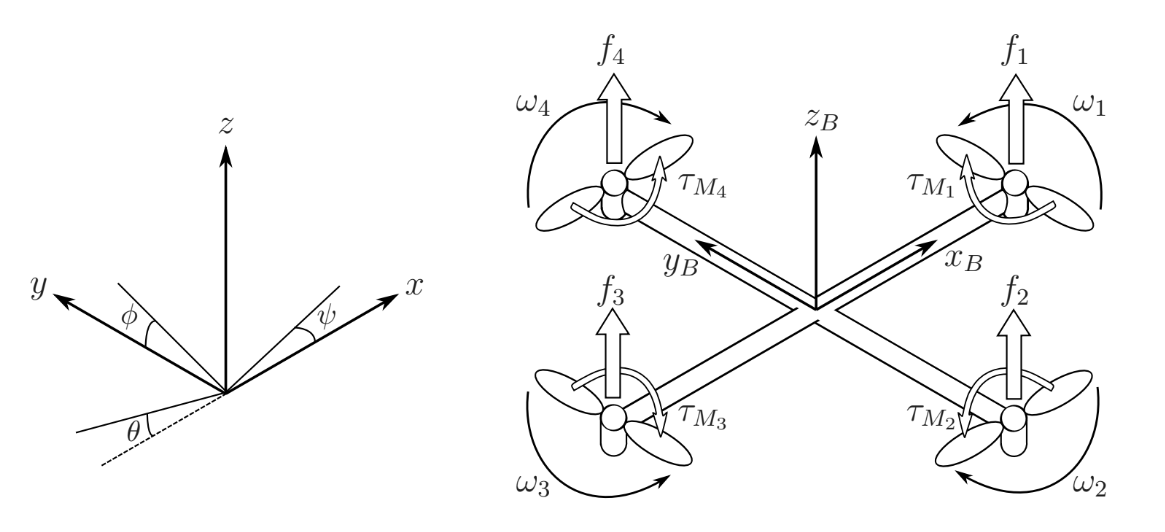
\includegraphics[width = 14cm]{pictures/drone-model.png}
            \caption{Diagrama de cuerpo libre de un quadc\'optero.}
            \label{fig:drone-model}
        \end{figure}

        La posición lineal absoluta del quadc\'optero se define como $\boldsymbol{\xi}$ y se mide a partir de los ejes $x$, $y$ y $z$. Posterior a ello se define la posici\'on angular en el marco inercial con un vector $\boldsymbol{\eta}$ compuesto por tres \'angulos de Euler $\phi$ (roll), $\theta$ (pitch) y $\psi$ (yaw). Roll determina la rotación con respecto al eje $x$, pitch con respecto al eje $y$ y yaw con respecto al eje $z$. El vector $\boldsymbol{q}$ contiene los vectores de las posiciones lineales y angulares.
    
        \begin{align}
            \boldsymbol{\xi} &= 
            \left[{
                \begin{array}{c}
                    x \\
                    y \\
                    z \\
                \end{array} 
            }\right],
            &\quad
            \boldsymbol{\eta} &= 
            \left[{
                \begin{array}{c}
                    \phi \\
                    \theta \\
                    \phi \\
                \end{array} 
            }\right],
            &\quad
            \boldsymbol{q} &=
            \left[{
                \begin{array}{c}
                    \boldsymbol{\xi} \\
                    \boldsymbol{\eta} \\
                \end{array} 
            }\right].
        \end{align}

        El origen del marco de referencia del cuerpo es el centro de masa del quadc\'optero. En el marco de referencia del cuerpo, las velocidades lineales se determinan por $\boldsymbol{V}_B$ y las velocidades angulares por $\boldsymbol{\nu}$.

        \begin{align}
            \boldsymbol{V}_B &= 
            \left[{
                \begin{array}{c}
                    v_{x,B} \\
                    v_{y,B} \\
                    v_{z,B} \\
                \end{array} 
            }\right],
            &\quad
            \boldsymbol{\nu} &= 
            \left[{
                \begin{array}{c}
                    p \\
                    q \\
                    r \\
                \end{array} 
            }\right].
        \end{align}

        La matriz de rotación del marco de referencia del cuerpo al inercial está dada por:

        \begin{equation}
            \boldsymbol{R} = 
            \left[{
                \begin{array}{ccc}
                    \cos{\psi}\cos{\theta}  & 
                    \cos{\psi}\sin{\theta}\sin{\phi} - \sin{\psi}\cos{\phi}    &
                    \cos{\psi}\sin{\theta}\cos{\phi} + \sin{\psi}\sin{\phi}    \\
                    \sin{\psi}\cos{\theta}  & 
                    \sin{\psi}\sin{\theta}\sin{\phi} - \cos{\psi}\cos{\phi}    &
                    \sin{\psi}\sin{\theta}\cos{\phi} + \cos{\psi}\sin{\phi}    \\
                    -\sin{\theta}           &
                    \cos{\theta}\sin{\phi}  &
                    \cos{\theta}\cos{\phi}  \\
                \end{array} 
            }\right]
        \end{equation}

        Se puede verificar que la matriz de rotación $\boldsymbol{R}$ es ortogonal teniendo que $\boldsymbol{R}^{-1} = \boldsymbol{R}^{\mathrm{T}}$, que corresponde al proceso inverso (matriz de rotación del marco de referencia inercial al del cuerpo). Por otra parte, la matriz de transformación de las velocidades angulares del marco de referencia inercial al del cuerpo se denota como $\boldsymbol{W}_{\eta}$. De la misma manera, la inversa de dicha matriz corresponde al proceso inverso. Por consiguiente, se obtiene que
    
        \begin{align}
            \begin{aligned}
                \boldsymbol{\dot{\eta}} &=
                \boldsymbol{W}_{\eta}^{-1}\boldsymbol{\nu},
                &\quad
                \left[{
                    \begin{array}{c}
                        \dot{\phi} \\
                        \dot{\theta} \\
                        \dot{\psi} \\
                    \end{array} 
                }\right] &= 
                \left[{
                    \begin{array}{ccc}
                        1 & \sin{\phi}\tan{\theta} & \cos{\phi}\tan{\theta}     \\
                        0 & \cos{\phi} & -\sin{\phi} \\
                        0 & \sin{\phi}/\cos{\theta} & \cos{\phi}/\cos{\theta} \\
                    \end{array} 
                }\right]
                \left[{
                    \begin{array}{c}
                        p \\
                        q \\
                        r \\
                    \end{array} 
                }\right],
                \\
                \boldsymbol{\nu} &=
                \boldsymbol{W}_{\eta}\boldsymbol{\dot{\eta}},
                &\quad
                \left[{
                    \begin{array}{c}
                        p \\
                        q \\
                        r \\
                    \end{array} 
                }\right] &= 
                \left[{
                    \begin{array}{ccc}
                        1 & 0 & -\sin{\theta}  \\
                        0 & \cos{\phi} & \cos{\theta}\sin{\phi} \\
                        0 & -\sin{\phi} & \cos{\theta}\cos{\phi} \\
                    \end{array} 
                }\right]
                \left[{
                    \begin{array}{c}
                        \dot{\phi} \\
                        \dot{\theta} \\
                        \dot{\psi} \\
                    \end{array} 
                }\right].
            \end{aligned}
        \end{align}

        La matriz $\boldsymbol{W}_{\eta}$ es invertible solo si $\theta\neq(2k-1)\phi/2,\;(k\in\mathbb{Z})$. Luego, debido a que se asume que el quadc\'optero tiene estructura sim\'etrica con los cuatro brazos alineados con el cuerpo en los ejes $x$ y $y$, el momento de inercia es la matriz diagonal $\boldsymbol{I}$ donde $I_{xx} = I_{yy}$, entonces

        \begin{equation}
            \boldsymbol{I} = 
            \left[{
                \begin{array}{ccc}
                    I_{xx} & 0 & 0 \\
                    0 & I_{yy} & 0 \\
                    0 & 0 & I_{zz} \\
                \end{array} 
            }\right].
        \end{equation}

        La velocidad angular del motor $i$, denotada como $\omega_i$, crea una fuerza $f_i$ en la direcci\'on del eje del motor. La velocidad angular y aceleraci\'on del rotor tambi\'en crean un torque $\tau_{M_i}$ alrededor del eje del motor, teniendo que
        \begin{align}
            f_i &= k\omega_i^2, & \tau_{M_i} &= b\omega_i^2 + I_M\dot{\omega}_i,
        \end{align}
        donde $k$ es la constante de elevaci\'on, $b$ es la constante de arrastre y $I_M$ es el momento de inercia del motor. En la mayor\'ia de los casos el efecto de $\dot{\omega}$ se considera pequeño y por ende se omite.

        Las fuerzas combinadas de los motores crean la fuerza de empuje $T$ en direcci\'on del eje $z$ del cuerpo. Igualmente, el torque total del cuerpo $\boldsymbol{\tau}_B$ se forma con los torques de cada \'angulo de Euler, siendo $\tau_{\phi}$, $\tau_{\theta}$ and $\tau_{\psi}$. Por ende,
        \begin{align}
            \sum_{i=1}^4 f_i &= k \sum_{i=1}^4 \omega_i^2, &\quad \boldsymbol{T}^B &= 
            \left[{
                \begin{array}{c}
                    0 \\
                    0 \\
                    T \\
                \end{array} 
            }\right],
            \label{eq:7}
        \end{align}
        \begin{equation}
            \boldsymbol{\tau}_B = 
            \left[{
                \begin{array}{c}
                    \tau_\phi \\
                    \tau_\theta \\
                    \tau_\psi \\
                \end{array} 
            }\right] = 
            \left[{
                \begin{array}{c}
                    lk\left(-\omega_2^2 + \omega_4^2 \right) \\
                    lk\left(-\omega_1^2 + \omega_3^2\right) \\
                    \sum_{i = 1}^{4}\tau_{M_i} \\
                \end{array} 
            }\right]
            \label{eq:8}
        \end{equation}
        donde $l$ es la distancia entre el motor y el centro de masa del quadc\'optero. Debido a que este se considera un cuerpo rígido, las ecuaciones de movimiento de Newton-Euler son usadas para describir su dinámica. En el marco de referencia del cuerpo, la fuerza requerida para la aceleraci\'on de una masa $m\dot{\boldsymbol{V}}_B$ y la fuerza centr\'ifuga $\boldsymbol{\nu}\times(m\boldsymbol{V}_B)$ son iguales a la gravedad $\boldsymbol{R}^T\boldsymbol{G}$ y la fuerza total de empuje de los motores $\boldsymbol{T}_B$, teniendo entonces que

        \begin{equation}
            m\dot{\boldsymbol{V}}_B + \boldsymbol{\nu}\times(m\boldsymbol{V}_B) = \boldsymbol{R}^T\boldsymbol{G} + \boldsymbol{T}_B.
        \end{equation}

        En el marco de referencia, la fuerza centrífuga se vuelve cero. Por lo tanto, \'unicamente la fuerza gravitacional y la magnitud y direcci\'on de la fuerza de empuje contribuyen en la aceleraci\'on del quadc\'optero, obteniendo que

        \begin{equation}
            \begin{gathered}
                m\boldsymbol{\ddot{\xi}} = \boldsymbol{G} + \boldsymbol{RT}_B, \\
                \left[{
                    \begin{array}{c}
                        \ddot{x} \\
                        \ddot{y} \\
                        \ddot{z} \\
                    \end{array} 
                }\right] = -g
                \left[{
                    \begin{array}{c}
                        0 \\
                        0 \\
                        1 \\
                    \end{array} 
                }\right] + \frac{T}{m}
                \left[{
                    \begin{array}{c}
                        \cos{\psi}\sin{\theta}\cos{\phi} + \sin{\psi}\sin{\phi} \\
                        \sin{\psi}\sin{\theta}\cos{\phi} - \cos{\psi}\sin{\phi} \\
                        \cos{\theta}\cos{\phi} \\
                    \end{array} 
                }\right].
            \end{gathered}
        \end{equation}

        En el marco de referencia del cuerpo, la aceleración angular del momento de inercia $\boldsymbol{I\dot{\nu}}$, las fuerzas centrípetas $\boldsymbol{\nu}\times(\boldsymbol{I\nu})$ y las fuerzas giroscópicas $\boldsymbol{\Gamma}$ son iguales al torque externo $\boldsymbol{\tau}$ de la siguiente manera:

        \begin{equation}
            \begin{gathered}
                \boldsymbol{I\dot{\nu}} + \boldsymbol{\nu}\times(\boldsymbol{I\nu}) + \boldsymbol{\tau}, \\
                \boldsymbol{\dot{\nu}} = -
                \left[{
                    \begin{array}{c}
                        p \\
                        q \\
                        r \\
                    \end{array} 
                }\right] \times 
                \left[{
                    \begin{array}{c}
                        I_{xx}p \\
                        I_{yy}q \\
                        I_{zz}r \\
                    \end{array} 
                }\right] - I_r
                \left[{
                    \begin{array}{c}
                        p \\
                        q \\
                        r \\
                    \end{array} 
                }\right] \times 
                \left[{
                    \begin{array}{c}
                        0 \\
                        0 \\
                        1 \\
                    \end{array} 
                }\right] \omega_{\Gamma} + \tau, \\
                \left[{
                    \begin{array}{c}
                        \dot{p} \\
                        \dot{q} \\
                        \dot{r} \\
                    \end{array} 
                }\right] = 
                \left[{
                    \begin{array}{c}
                        (I_{yy} - I_{zz})qr/I_{xx} \\
                        (I_{zz} - I_{xx})qr/I_{yy} \\
                        (I_{xx} - I_{yy})qr/I_{xx} \\
                    \end{array} 
                }\right] - I_r
                \left[{
                    \begin{array}{c}
                        q/I_{xx} \\
                        -p/I_{yy} \\
                        0 \\
                    \end{array} 
                }\right] \omega_{\Gamma} + 
                \left[{
                    \begin{array}{c}
                        \tau_{\phi}/I_{xx} \\
                        \tau_{\theta}/I_{yy} \\
                        \tau_{\psi}/I_{zz} \\
                    \end{array} 
                }\right],
            \end{gathered}
        \end{equation}
        donde $\omega_{\Gamma} = \omega_1 - \omega_2 + \omega3 - \omega4$. Este modelo es implementado en MATLAB®/Simulink™ y a continuación se explica su sistema de control.

        \subsection{Sistema de Control del Quadc\'optero}\label{sec3.2}
        Ahora bien, para estabilizar el quadc\'optero se propone emplear un controlador PID cuya estructura se define como
        \begin{equation}
            u(t) = K_Pe(t) + K_I\int_0^t e(\tau) d\tau + K_D \frac{de(t)}{dt}
        \end{equation}
        donde $u(t)$ es la salida del controlador, $e(t)$ se define como el error, es decir, la diferencia entre el estado deseado y el estado presente. Los parámetros $K_P$, $K_I$ y $K_D$ son los coeficientes proporcional, integral y derivativo que ayudar\'an a sintonizar el controlador PID, respectivamente. Para realizar el modelo, se debe considerar que a pesar de que se tienen seis estados, siendo estos tres posiciones y tres \'angulos, se consideran \'unicamente cuatro entradas de control, que corresponden a las velocidades angulares de los cuatro motores. La fuerza de empuje total $T$ afecta la aceleración en la dirección del eje $z$ y mantiene al dron en el aire. Asimismo, los torques afectan la aceleración de los ángulos roll, pitch y jaw. Habiendo descrito esto, la propuesta del controlador se describe como

        \begin{equation}
            \begin{gathered}
                T = \left[g + K_{z,P}\;e_z + K_{z,I}\int_0^t{e_z\;d\tau} + K_{z,D}\;\dot{e_z}\right]\cdot\frac{m}{\cos{\phi}\cos{\theta}} 
                \\
                \tau_{\phi} = \left[K_{\phi,P}\;e_\phi + K_{\phi,I}\int_0^t{e_\phi\;d\tau} + K_{\phi,D}\;\dot{\phi_z}\right]\cdot I_{xx} 
                \\
                \tau_{\theta} = \left[K_{\theta,P}\;e_\theta + K_{\theta,I}\int_0^t{e_\theta\;d\tau} + K_{\theta,D}\;\dot{e_\theta}\right]\cdot I_{yy} 
                \\
                \tau_{\psi} = \left[K_{\psi,P}\;e_\psi + K_{\psi,I}\int_0^t{e_\psi\;d\tau} + K_{\psi,D}\;\dot{e_\psi}\right]\cdot I_{zz} \\
            \end{gathered}
            \label{eq:13}
        \end{equation}

        La velocidad angular de los motores es despu\'es calculada con las Ecuaciones (\ref{eq:7}) y (\ref{eq:8}) con los valores obtenidos en la ecuaci\'on (\ref{eq:13}) de la siguiente manera:

        \begin{equation}
            \begin{gathered}
                \omega_1^2 = \frac{T}{4k} - \frac{\tau_\theta}{2kl} - \frac{\tau_\psi}{4b}
                \\
                \omega_2^2 = \frac{T}{4k} - \frac{\tau_\phi}{2kl} + \frac{\tau_\psi}{4b}
                \\
                \omega_3^2 = \frac{T}{4k} + \frac{\tau_\theta}{2kl} - \frac{\tau_\psi}{4b}
                \\
                \omega_4^2 = \frac{T}{4k} + \frac{\tau_\phi}{2kl} + \frac{\tau_\psi}{4b}
            \end{gathered}
        \end{equation}

        Este control es implementado en MATLAB®/Simulink™ junto con el modelo anterior.

    \section{Resultados}\label{sec4}

    \section{Conclusiones}\label{sec5}

    \printbibliography

\end{document}